\chapter{Particle system}
\label{cha:particlesystem}

Particle system is one of most commonly used techniques to simulate smoke, fire, rain and other groups of discrete objects, usually independent from each other. The system consists of a defined number of emitters, producing lightweight particle objects with certain parameters. Each emitter has a defined production ratio, and each particle a certain lifespan, resulting in the upper limit of total particles on the screen. Some systems also use attraction points, which enable better control over particles, using equations often similar to those of electrostatic forces.
Such simulation is independent from rendering. The same particle system can be used for different effects with proper configuration.

\begin{figure}[h!]
  \caption{Example rendering of tested particle system}
  \label{img:particles}
  \centering
	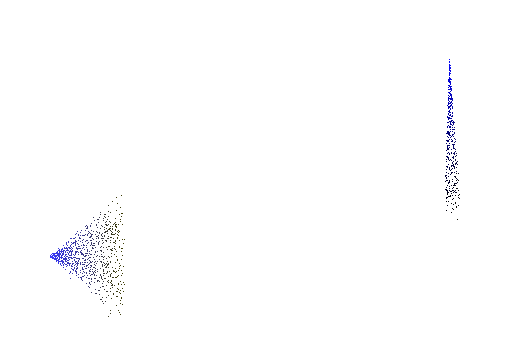
\includegraphics[width=16cm]{particles}
\end{figure}

\section{System parameters}
\label{sec:emittersparameters}

The tested system works on the two-dimensional Cartesian plane. For the purpose of performance analysis, movements are calculated based only on frames rather than actual flow of time. This means that systems with a different framerate will result in different visualisations, but requesting a given amount of frames rendered will result in the same lifespan and total number of particles in both systems.

Emitter supports the following parameters:

\begin{itemize}
	\item position -- initial position of created particles
	\item angle -- angle counting clockwise from the vector [0, 1]
	\item spread -- parameter controlling random differences in the initial angle of particles
	\item velocity -- initial velocity of particles, in pixels per frame
	\item velocity spread -- parameter controlling random differences in the initial velocity of particles
	\item lifespan -- initial lifespan of particles
	\item productionRate -- amount of particles initialized in each frame
\end{itemize}

A Particle has similar properties:
\begin{itemize}
	\item position
	\item velocity
	\item lifespan
	\item age -- counted in frames, when for given particle it is higher than its lifespan, particle is removed from the system
\end{itemize}

Source code of both implementations is attached in the Appendix \ref{cha:sourcecode}.

\section{Implementation with high memory allocation}
\label{sec:particlesinitial}

The initially tested implementation has one very important property of a particle emitter. Whenever new particles are created, a new array of pointers is allocated and returned from the emitter. The system appends new particles to the existing array. In each frame, the particle system creates a new, empty array of particles and adds only particles that are still alive. The array from the previous frame and all dead particles are removed from the system and deallocated. This is clearly a suboptimal solution that allocates and deallocates plenty of memory in each frame. The purpose of this exercise is to show how both languages handle a bad code, and how big impact it has compared to the optimal solution.

\lstinputlisting[caption=Time measurement of unoptimized particle system in JavaScript,label=listing:timejs1]{particles/timejs1.txt}
\lstinputlisting[caption=Time measurement of unoptimized particle system in C++,label=listing:timecpp1]{particles/timecpp1.txt}

Time measurement shows that the JavaScript version is almost 8 times slower than the native one. To analyse the situation --prof and --log-timer-events flags may be used. The output file v8.log is parsed using an available online tool.\cite{v8-profile-plotter}

\lstinputlisting[caption=Profiler output for unoptimized particles,label=listing:particles1profile]{particles/particles1-profile.txt}

Methods prefixed with ~ are unoptimized, the ones prefixed with * are JIT compiled. As seen in the profiler log, most of the time is spent in unoptimised versions of verifyIfAlive and stepParticle methods.

\lstinputlisting[caption=Annotated part of source,label=listing:particles1stepannotated,language=JavaScript]{particles/particleSystemstep.js}

The same methods are also used in optimised versions, where they take significantly less ticks to run. It is clear that the presented code not only allocates and deallocates too much memory, but also fails to run in optimised mode. It is visible on the chart obtained from the same tool -- stripe labelled "code kind in execution" shows multiple kinds of code running and is interrupted often with garbage collection cycles.

\begin{figure}[h!]
  \caption{Chart of time used in unoptimised verion of JavaScript}
  \label{img:particles1profile}
  \centering
	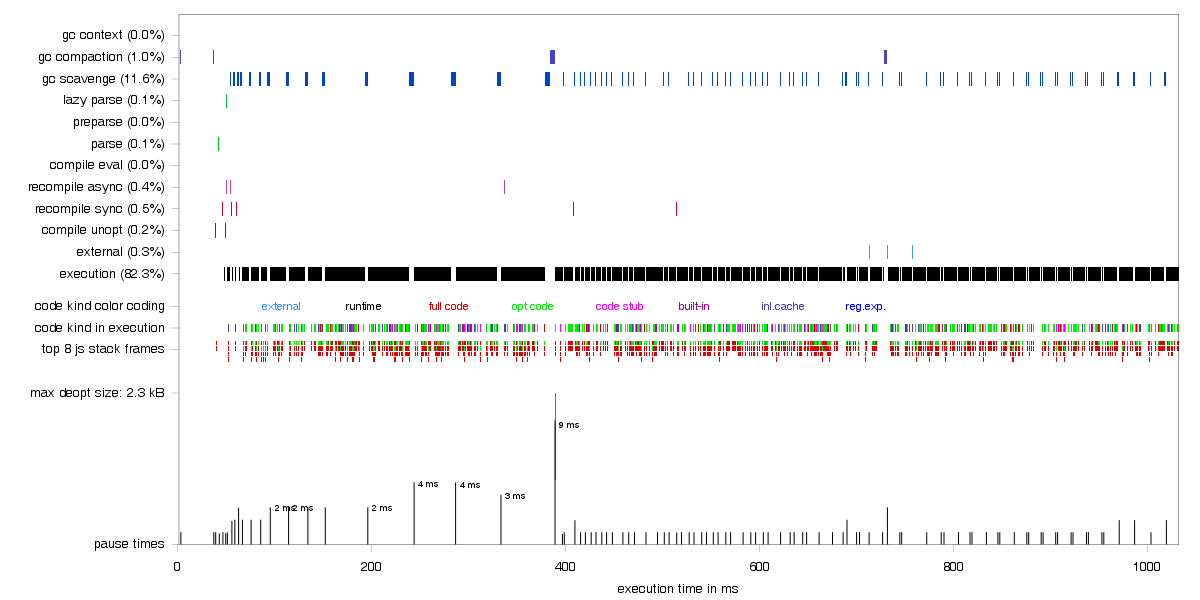
\includegraphics[width=16cm]{particles/particles1-profile.png}
\end{figure}

Garbage collection cycles blocking execution are also visible with --trace-gc flag.

\lstinputlisting[caption=Garbage collection in unoptimised particle system,label=listing:particles1gc]{particles/particles1gc.txt}

\section{Implementation with object pool}
\label{sec:particlesobjectpool}

To improve performance, a different approach to particles allocation is used. Each particle has a flag "isDead" telling if it may be safely reused for a new particle. The particle pool is kept along with a list of pointers to dead particles. This way, when the system reaches its maximum congestion (around 15000 particles in the given example) no new allocations occur.
The creation of new particles is moved from the particle emitter to the particle system, to avoid allocation of the new array. The emitter works now as a structure describing behaviour, but not implementing one.

\lstinputlisting[caption=Time measurement of optimized particle system in JavaScript,label=listing:timejs2]{particles/timejs2.txt}
\lstinputlisting[caption=Time measurement of optimized particle system in C++,label=listing:timecpp2]{particles/timecpp2.txt}

The optimised version shows overall improvement of 85\% for JavaScript and 45\% for C++ making the JavaScript version only 2.2 times slower than the native one. It is clearly visible that JavaScript is more sensitive to unwise memory management.

\lstinputlisting[caption=Profiler output for optimized particles,label=listing:particles1profile]{particles/particles2-profile.txt}

Profiling shows that the step method of the particle system is now always running in optimised mode, and almost no time is spent on other methods. The same is visible on the profiling chart, where the "code kind in execution" stripe shows only the optimised code.

\begin{figure}[h!]
  \caption{Chart of time used in optimised verion of JavaScript}
  \label{img:particles2profile}
  \centering
	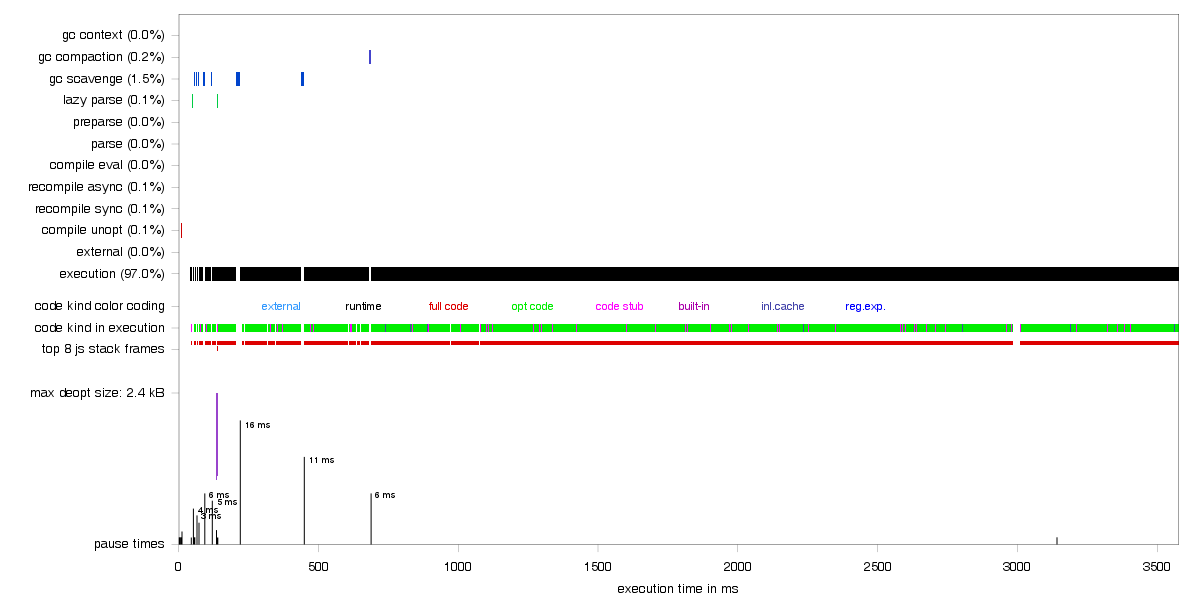
\includegraphics[width=16cm]{particles/particles2-profile.png}
\end{figure} 

The situation has also improved in the garbage collection log.

\lstinputlisting[caption=Garbage collection in optimised particle system,label=listing:particles2gc]{particles/particles2gc.txt}
